\documentclass[article,
12pt,
a4paper,
openany,
oneside,
brazil,
]{abntex2}

\usepackage[brazil]{babel}
\usepackage[
  left=3cm,
  top=3cm,
  right=2cm,
  bottom=2cm, 
]{geometry}
\usepackage{caption}
\usepackage{indentfirst}
\usepackage{graphicx}
\usepackage{xcolor}
\usepackage{microtype} 			% para melhorias de justificação
\usepackage[alf, 
  abnt-emphasize = bf,
  abnt-etal-list = 2,
  abnt-etal-cite = 2,
  bibjustif,
  abnt-etal-text=default
  % abnt-etal-text=it
]{abntex2cite}	% CITAÇÕES PADRÃO ABNT
\usepackage{fontspec}
\usepackage{url}
\usepackage{fancyhdr}
\usepackage{ragged2e}
\usepackage{listings}



\setmainfont{Arial}

% O tamanho do parágrafo(recuo) é dado por:
\setlength{\parindent}{1.25cm}
\linespread{1.5}

\selectlanguage{brazil}

\makeatletter
\hypersetup{
      pdftitle={\@title}, 
		  pdfauthor={\@author},
	    pdfcreator={Hugo Soares},
      pdfkeywords={OpenCV}{Template Matching},
  		colorlinks=true,
    	citecolor=black,
      linkcolor=black,
      urlcolor=black,
	    bookmarksdepth=4
}

\NewDocumentCommand{\codeword}{v}{%
\texttt{\textcolor{blue}{#1}}%
}


\titulo{Relatorio Final}

\autor{Hugo Oliveira Soares \\ E01381}
\orientador{}
\coorientador{}

\local{Belo Horizonte}
\instituicao{Dom Helder Escola Superior}
\data{2023}

\makeindex

\begin{document}

  % PARTE PRÉ-TEXTUAL
  \maketitle

  % PARTE TEXTUAL
  \textual
  \pagenumbering{arabic}

  %TODO: Explicar pq está usando um algoritmo em detrimento do outro

  \section{Template Matching}
    Template Matching é um método para encontrar uma imagem (template) dentro de outra imagem maior(origem). O \textit{OpenCV} vem com uma função \codeword{cv.matchTemplate()} para está finalidade.

    O algoritmo compara o template com a imagem de entrada ``deslizando" uma sobre a outra, movendo um pixel de cada vez(da esquerda para a direita, de cima para baixo), calculando o quão proximo é a correspondência nessa area \cite{ana}.

    \begin{figure}[!htbp]
      \center
      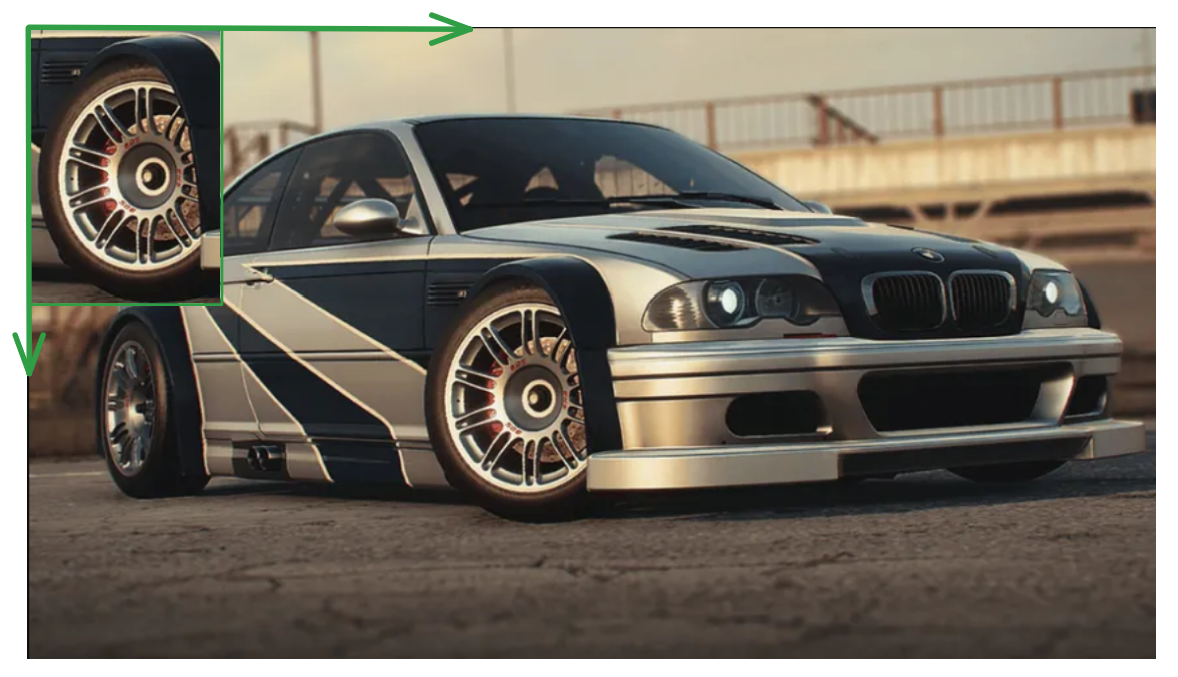
\includegraphics[scale=0.4]{compara.png}
      \caption{Comparação entre a imagem template e a imagem origem}
    \end{figure}

    \newpage
    Para a comparação o OpenCV tem diversos métodos, dentre eles são:
    \begin{itemize}
      \item cv.TM\_CCOEFF 
      \item cv.TM\_CCOEFF\_NORMED 
      \item cv.TM\_CCORR
      \item cv.TM\_CCORR\_NORMED
      \item cv.TM\_SQDIFF
      \item cv.TM\_SQDIFF\_NORMED
    \end{itemize} 


  \section{Corner Detection}
    Conner Detection é um método para identificar pontos distintos ou cantos em uma imagem. Um canto é um ponto onde a vizinhança local está em duas direções diferentes. Um canto pode ser definido como a intercessão de duas bordas.

  \section{Canny Edge Detection}
  \section{Face Detection with Haar Cascades}
  % Referencias
  \newpage
  \bibliography{referencias}

\end{document}
